\documentclass[tc, manuscript]{copernicus}

\usepackage{booktabs}
\usepackage{multirow}
\usepackage{siunitx} %for SI units

\begin{document}

\title{Fountain scheduling strategies to improve water use efficiency of artificial
ice reservoirs (Icestupas)}

\def\Authors{Suryanarayanan Balasubramanian\,$^{1,2}$, Martin Hoelzle\,$^{1}$Roger Waser\,$^{3}$,}

\def\Address{$^{1}$University of Fribourg, Department of Geosciences, Fribourg, Switzerland $^{2}$University of
Applied Sciences and Arts, Luzern, Switzerland} \def\corrAuthor{Suryanarayanan Balasubramanian}
\Author[1,2]{Suryanarayanan}{Balasubramanian}
\Author[1]{Martin}{Hoelzle}
\Author[3]{Roger}{Waser}
% \Author[3]{Martin}{Von Burg}
\affil[1]{University of Fribourg, Department of Geosciences, Fribourg, Switzerland}
\affil[2]{Himalayan Institute of Alternatives, Ladakh, India}
\affil[3]{University of Applied Sciences and Arts, Luzern, Switzerland}

\correspondence{suryanarayanan.balasubramanian@unifr.ch}

\runningtitle{Scheduling AIR fountains}

\runningauthor{S. Balasubramanian}

\firstpage{1}

\maketitle

\begin{abstract}

  Artificial Ice Reservoir (AIR), often also called - Ice Stupa - are a climate adaptation strategy developed in
  the Indian Himalayas (Ladakh). With this technology, otherwise unused stream or lake water is stored in large
  ice towers in winter. The surplus melt water that is then available in spring is used for satisfying
  irrigation water demands. Recent studies have shown that during construction of traditional AIRs over 75 \% of
  the water sprayed was lost. Therefore, fountain wastewater production have to be reduced to improve water use
  efficiency. Improved fountain scheduling was realized using an automation system that computes recommended
  discharge rates using real-time weather inputs and location metadata. During the winter of 2021-22, a
  traditional and an automated AIR were built in Guttannen, Canton of Berne, Switzerland with the main aim of
  comparing and quantifying the benefits of fountain scheduling through automation systems. The scheduled
  fountain produced similar ice volumes while consuming 87 \% lesser water than the unscheduled fountain.
  Overall, these results show that scheduled fountains can increase the water use efficiency without
  compromising on meltwater production.

\end{abstract}

\introduction

In some arid mountain regions the lack of water during the irrigation season is the main constraint on
agricultural production. Recently, an increasing need of irrigation water supply has prompted more than 30
villages in Ladakh, India to construct artificial ice reservoirs (AIRs) or icestupas. These AIRs are
traditionally constructed by diverting springs, glacial streams or lakes into fountain spray systems via
embankments and pipelines. However, there is a large variability associated with this water supply due to the
local weather influences and discharge rate of the chosen location and fountain respectively. 

Previous studies (\citep{balasubramanianInfluenceMeteorologicalConditions2022},
\citep{oerlemansBriefCommunicationGrowth2021}) have already quantified the meteorological influences on AIR
volume evolution by comparing several AIRs built in India and Switzerland. The results of these previous study
revealed the high sensitivity of AIR volume evolution on the fountain characteristics. Moreover, it was found
that all the AIRs constructed suffered from very high water losses due to excessive fountain discharge input. 

A straightforward solution to this issue is to reduce the fountain discharge input but it is challenging to
implement it in practice. For example, in the case of the Indian AIR, the model estimates that water use
efficiency can be increased without compromising the ice volume by just reducing the fountain discharge rate by
half. However, in practice, this strategy would have further increased the number of pipeline freezing events
due to much lower water velocities in the pipeline. 

An optimum construction strategy, therefore, should prevent pipeline freezing events while maintaining high
water use efficiency. Typical solutions to prevent pipeline freezing events given pipeline dimensions and
discharge rates are to bury or drain the pipeline. Burying the pipeline at a sufficient depth can reduce the
influence of atmospheric conditions on the pipeline water temperature. Even though this method is ideal, it can
quickly get expensive depending on the length of the pipeline and the frost depth. Therefore, such an effort is
warranted only in the case of a permanent construction location. Comparatively, draining the pipeline is a much
cheaper strategy. Moreover, it can be combined with fountain scheduling methods to achieve reduced watering
volumes for AIR construction systems.

Proper fountain scheduling requires answers to two questions: 
(a) When should the water be turned on and off ?
(b) How much water should be sprayed ? 

For answering these questions, knowledge of surface freezing rates is important . Surface freezing rates can be
calculated by means of the full energy balance model developed in
\cite{balasubramanianInfluenceMeteorologicalConditions2022}. This model can be forced with either historical
weather data or real-time weather data to produce recommended discharge rates. We further approximate the model
by including two kinds of assumptions that are considerate for the limited water availability or the favourable
weather windows respectively.

However, manually adjusting the fountain discharge rate is unrealistic. Firstly, constant adjustments of
discharge rates in response to the significant diurnal and seasonal variations of the freezing rates is
impractical. Secondly, frequent pipeline water drainage required to prevent freezing events during critical weather
windows is unfeasible. Therefore, operation of scheduled fountains via automation systems is preferred.

The present study builds upon previous work \citep{balasubramanianInfluenceMeteorologicalConditions2022}, in
order to quantify the influence of different fountain scheduling strategies on the mass and energy balance of
AIRs with identical meteorological conditions. The main interest in using model results is to simulate fountain
schedules relative to constraints in favourable weather windows and water availability. The fountain
scheduling strategies are evaluated from the relative water use efficiency and maximum ice volume produced
during the study period. The specific objectives of this paper include the mass and energy balance
comparison of fountain scheduling strategies, presentation of the automation system, and examples of its
application to the computation of fountain scheduling strategies.

\section{Study site and data}

The Guttannen site (46.66 $\degree$N, 8.29 $\degree$E) is situated in the Berne region, Switzerland and has an
altitude of 1047 $m$ a.s.l. In the winter (Oct-Apr), mean daily minimum and maximum air temperatures vary
between -13 and 15 $\degree C$. Clear skies are rare, averaging around 7 days during winter. Daily winter
precipitation can sometimes be as high as 100 $mm$. These values are based on 30 years of hourly weather model
simulations \citep{guttannen}. Two AIRs were constructed by the Guttannen Bewegt Association, the University of
Fribourg and the Lucerne University of Applied Sciences and Arts during the winters of 2021-22 using a
traditional and an automated construction strategy.

\begin{figure}[t]
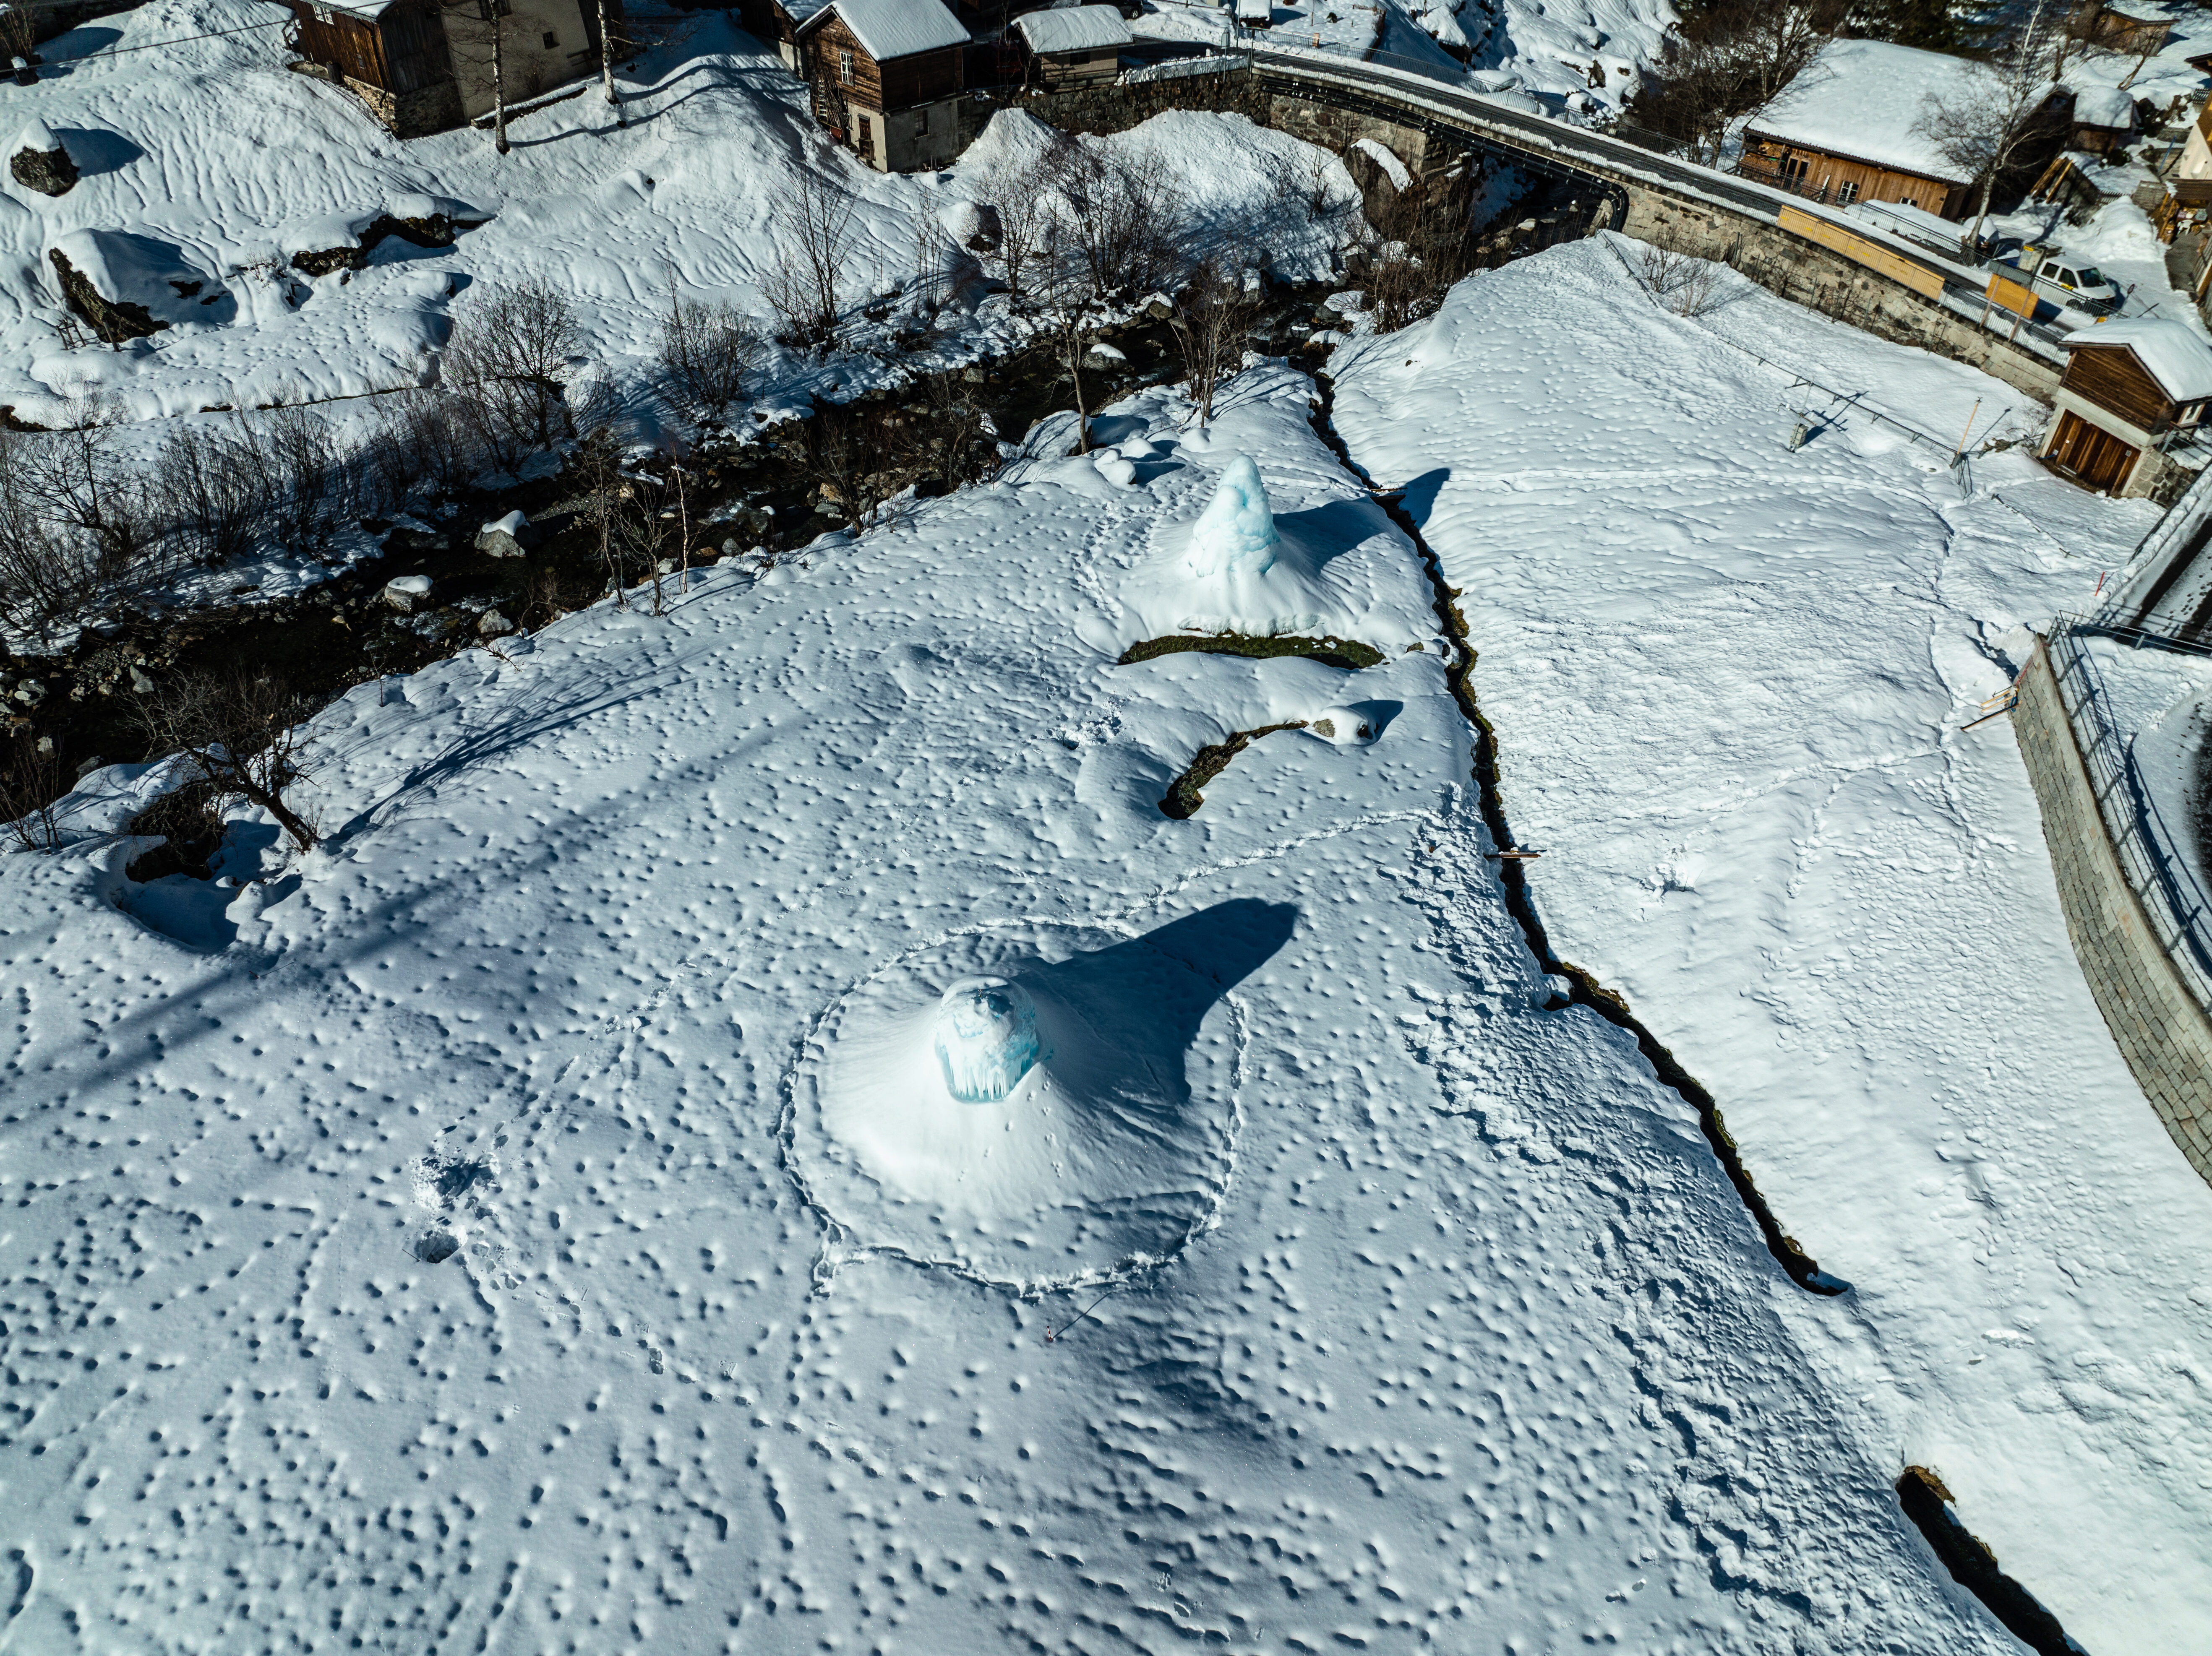
\includegraphics[width=8.3cm]{Figures/2AIRs.jpg}
\caption{Automated and traditional AIRs  at Guttannen on February 6, 2022. Picture credits: Daniel Bürki}
\label{fig:2AIR} 
\end{figure}

The automated and the traditional AIRs were constructed adjacent to each other as shown in Fig. \ref{fig:2AIR}.
This ensured both AIRs shared the same water source and similar weather conditions. In addition, a webcam
guaranteed a continuous survey of the automated AIR.   

In the traditional strategy, tree branches were laid covering the fountain pipe to initiate and speed up the ice
cone formation process. The fountain discharge was maintained at maximum and its height was increased from 3 to
6\,$m$ during the construction period.

In the automated strategy, only the fountain pipe was placed before the water spray started. A programmed
automation system controlled the fountain discharge rate during the whole winter season using real time weather
input and several control parameters, which could be tested and controlled via a data logger user interface. 

\subsection{Meteorological data}

Air temperature, relative humidity, wind speed, pressure, longwave, shortwave direct and diffuse radiation are
required to calculate the surface energy balance of an AIR (see Fig. \ref{fig:aws}). The construction period
starts when the fountain was first switched on and ends when the fountain was last switched off. These two dates
are denoted as start and fountain off dates henceforth.

\begin{figure*}[t]
\includegraphics[width=12cm]{Figures/data.png}
\caption{Temperature, precipitation and discharge measurements at the Guttannen construction site}
\label{fig:aws} 
\end{figure*}

The weather data source was an automatic weather station (AWS) located around 20 m away as shown in Fig.
\ref{fig:2AIR}. Less than 0.4 \% of the data was found to be corrupted and these were filled by linear
interpolation. We define the fountain used through four attributes by the spray radius, the discharge rate, the
pipe height and the water temperature.

\subsection{Fountain observations}

The spray radius $r_F$ was estimated from the mean AIR circumference measured in the drone surveys during the
fountain runtime. The discharge rate and water temperature of the scheduled fountain was measured by the
automation system but no such datasets were recorded for the unscheduled fountain. The unscheduled fountain was
operated at the maximum discharge rate using the same water source. Therefore, the maximum recorded discharge
rate and water temperature dataset of the scheduled fountain was used to estimate the corresponding variables of
the unscheduled fountain. The discharge rate of both fountains decreased with increase in its fountain pipeline
height. We observed a reduction in the scheduled fountain's maximum discharge rate by a factor of two whenever
the height was increased by a meter. The same reduction in magnitude was also applied for the unscheduled
fountain's discharge rate whenever pipeline height increase events occurred. A new fountain design was used for
the automated strategy since the traditional fountain design was unable to function in the whole range of
discharge rates suggested by the automation system.

\subsection{Drone surveys}

Several photogrammetric surveys were conducted on the traditional and the automated AIRs. The details of these
surveys and the methodology used to produce the corresponding outputs are explained in the Appendix. The digital
elevation models (DEMs) generated from the obtained imagery were analysed to document the spray radius, the
surface area and the volume of the ice structures. The number of drone surveys conducted for the traditional and
the automated AIRs were 6 and 3, respectively (see Table). The last drone flight was used to set the dome volume
for the traditional AIR. The dome volume for the automated AIR represented the snow volume found before the
fountain was switched on. The remaining surveys were used for model validation.

\begin{table}
	\centering
	\caption{ Summary of the drone surveys}
	\label{tab:uav}
	\begin{tabular}{@{}|llllll|@{}}
		\toprule
		\textbf{}              & \textbf{No.} & \textbf{Date} & \textbf{Volume} & \textbf{Radius} & \textbf{Surface Area} \\ \midrule
		\multicolumn{1}{|l|}{\multirow{6}{*}{\rotatebox[origin=c]{90}{Traditional}}}
		                       & 1            & Dec 23, 2021  & 17 $m^{3}$     & 2.9 $m$
		                       & 47 $m^{2}$                                                                      \\
		\multicolumn{1}{|l|}{} & 2            & Jan 3, 2022  & 22 $m^{3}$     & 3.4 $m$
		                       & 61 $m^{2}$                                                                      \\
		\multicolumn{1}{|l|}{} & 3            & Jan 22, 2022   & 626 $m^{3}$     & 4 $m$
		                       & 79 $m^{2}$                                                                      \\
		\multicolumn{1}{|l|}{} & 4            & Feb 6, 2022  & 44 $m^{3}$     & 4.2 $m$
		                       & 86 $m^{2}$                                                                      \\
		\multicolumn{1}{|l|}{} & 5            & Feb 12, 2022  & 62 $m^{3}$     & 4.2 $m$
		                       & 108 $m^{2}$                                                                      \\
		\multicolumn{1}{|l|}{} & 6            & & $m^{3}$     & $m$
		                       & $m^{2}$
		\\\midrule
		\multicolumn{1}{|l|}{\multirow{3}{*}{\rotatebox[origin=c]{90}{Automatic}}}
		                       & 1            & Dec 23, 2021  & 22 $m^{3}$      & 3.7 $m$
		                       & 57 $m^{2}$                                                                       \\
		\multicolumn{1}{|l|}{} & 2            & Jan 3, 2022   & 30 $m^{3}$      & 3.9 $m$
		                       & 66 $m^{2}$                                                                       \\
		\multicolumn{1}{|l|}{} & 3            &               &    $m^{3}$      &     $m$
		                       &    $m^{2}$                                                                       \\
		\bottomrule
	\end{tabular}

\end{table}

\section{Methods}

\subsection{Automation system}

\subsubsection{Automation hardware}

The automation hardware consists of an AWS, flowmeter, control valve, drain valves, air valves, fountain,
pipeline and a logger. The logger feeds the AWS data to the automation software and informs the recommended
discharge rate to the flowmeter. The flowmeter adjusts the control valve to match the recommendation. However,
the recommended discharge rate is ignored if any of the termination criterion are valid. The termination
criterion prevent water loss and pipeline freezing events. In case a termination criteria is valid, the drain
and air valves empty the water in the pipeline.

\subsubsection{Automation software}

Any construction location can either be constrained by the available water supply or the duration of favourable
weather windows for fountain operation. If the respective location has limited water supply then the fountain
scheduling strategy should be optimised for high water use efficiency (WUE). But if the location is limited by
the time period when the fountain can function then the scheduling strategy should be optimised for high ice
volumes (ICV).

Accordingly, we introduce two kinds of approximations in the automation software that optimise for the ICV and
WUE objective respectively. We approximate the expected (a) AIR shape using its slope parameter, (b) AIR surface
properties using its surface albedo and (c) weather conditions using the cloudiness parameter. The model
assumptions overestimate and underestimate the freezing rate for the ICV and WUE objectives respectively. These
assumptions are summarised in Table \ref{tab:assumptions}. 

\begin{table}[]
\centering
\caption{Assumptions introduced to simplify the model.}
\label{tab:assumptions}
\begin{tabular}{@{}lllll@{}}
\toprule
\textbf{Estimation of} & \textbf{Symbol} & \textbf{ICV Assumptions} & \textbf{WUE Assumptions} & \\ \midrule
\multicolumn{1}{|l}{AIR slope}        & $s_{cone}$ & $ 1 $ & $0$ & \multicolumn{1}{l|}{} \\ \midrule
\multicolumn{1}{|l}{Albedo} & $\alpha$ & $\alpha_{snow}$ & $\alpha_{ice}$ & \multicolumn{1}{l|}{} \\\midrule 
\multicolumn{1}{|l}{Cloudiness}  & $cld$ & $0$ & $1$ & \multicolumn{1}{l|}{} \\ \bottomrule
\end{tabular}
\end{table}

We apply the assumptions described in Table \ref{tab:assumptions} on the one-dimensional description of energy
fluxes as used in \cite{balasubramanianInfluenceMeteorologicalConditions2022} to obtain the rate of change of
AIR ice mass as follows: 

\begin{equation}
  \frac{\Delta M_{ice}}{\Delta t}  =  (\frac{q_{SW} + q_{LW} + q_{S} + q_{F} + q_{G} - q_{T}}{L_F} + \frac{q_{L}}{L_V} ) \cdot A_{cone}
	\label{eqn:auto}
\end{equation}

Upward and downward fluxes relative to the ice surface are positive and negative, respectively. The first term
represents the mass change rate due to freezing of the fountain water and melting of the ice. $q_{SW}$ is the
net shortwave radiation; $q_{LW}$ is the net longwave radiation; $q_{L}$ and $q_{S}$ are the turbulent latent
and sensible heat fluxes; $q_{F}$ is the fountain heat flux; $q_{G}$ is the ground heat flux; $q_{T}$ is the
temperature heat flux and $A_{cone}$ is the area of the AIR surface. The derivation of these individual terms
using the assumptions are discussed in the Appendix.

Equation \ref{eqn:auto} is implemented in the automation system through a user interface that enables input of
the spray radius, altitude, latitude and longitude of the construction location. Once switched on, the
automation system regulates the fountain discharge rate based on the recommended discharge rate. The recommended
discharge rate is equal to the ice mass change rate. However, certain termination criterias override the
discharge rate recommendation and drain the pipeline to prevent water loss or pipeline freezing events, namely: 

\begin{itemize}

\item High water loss is assumed if wind speed greater than critical wind speed.

\item High risk of pipeline freezing event is assumed if temperature lower than minimum fountain temperature.

\item High risk of pipeline freezing event is assumed if mass change rate is lower than minimum fountain discharge rate. 

\item Pipeline freezing events are assumed if $Q_F = 0$ for at least 20 seconds and the pipeline is drained as a
  consequence.

\item Pipeline leakage is assumed if discharge rate is greater than maximum fountain discharge rate.

\end{itemize}

\subsection{Calibration}

We retain the default values of all parameters used in
\cite{balasubramanianInfluenceMeteorologicalConditions2022} for our analysis.  

In addition, two model variables, fountain water temperature ($T_F$) and AIR density ($\rho_{AIR}$) are
parametrised. Both variables were assumed to be constant in the previous versions of the model. 

It is inaccurate to assume AIR density to be that of ice since the CH22 AIR had a significant mass contribution
in the form of snowfall. We instead parameterised AIR density $\rho_{AIR}$ as follows:

\begin{equation}
  \rho_{AIR} = \frac{M_{F} + M_{dep} + M_{ppt}}{(M_{F} + M_{dep})/\rho_{ice} + M_{ppt}/\rho_{snow}}
\end{equation}

where $M_F$ is the cumulative mass of the fountain discharge; $M_{ppt}$ is the cumulative precipitation; $M_{dep}$ is the cumulative accumulation through water vapour deposition; $\rho_{ice}$ is the ice density (917 $kg\,m^{-3}$) and $\rho_{snow}$ is the density of wet snow (300 $kg\,m^{-3}$) taken from
\cite{cuffeyPhysicsGlaciers2010} .

Also, a better fountain water temperature parameterisation is desired to accurately distinguish between the
fountain water heat flux of different scheduling strategies. With the extended measurement dataset of CH22 AIR,
we estimate the water temperature variable by assuming it is equal to our water temperature measurements but
only when the air temperature was not below the water temperature. Otherwise the water droplets are assumed to
cool to the ambient air temperature. Additionally, under subzero conditions, the water droplets are likely to
cool to 0 C during their flight time. Therefore, the fountain water temperature was instead determined as
follows:

\begin{equation}
	T_{F} = \left\{ \begin{array}{ll}
		0 & \textit{ if } T_{a} < 0 \\
		T_a & \textit{ if } T_{F} > T_a \\
		T_{F} & \textit{ otherwise}
	\end{array} \right.
\end{equation}

where $T_{F}$ is the measured fountain water temperature.


\subsection{Validation}

We performed the validation of the model on the traditional and automated AIRs by evaluating the root mean
squared error (RMSE) between ice volume estimates and measurements . Even though the number of drone flights
were identical for both AIRs, fewer successful volume observations were possible for the automated AIR as shown
in Table \ref{tab:uav}. This was because the DEMs generated for the automated AIR could not georeference the
automated AIR's snow covered surface. Since the traditional AIR was steeper, its surface revealed ice patches
that could be georeferenced. Root mean squared error (RMSE) served as the evaluation metric in both the cases.

The performance of the ICV and WUE versions of the physical model was assessed by comparing correlation of its
discharge rate estimates with the validated freezing rate of the calibrated physical model.

\section{Results}

\subsection{Energy balance model validation}
The physical model achieved an RMSE of $4 \degree C$ with the AIR mean temperature measurements of the automated AIR and an RMSE of $m^3$ with the ice volume measurements of the traditional AIR. The estimated and measured AIR
mean temperatures and ice volumes are shown in Fig. \ref{fig:validation}
 
\begin{figure*}[t] 
  \includegraphics[width=12cm]{Figures/validation.png} 
  \caption{Ice volume validation of the scheduled and unscheduled fountain construction strategies.} 
\label{fig:validation} 
\end{figure*}

\subsection{Scheduled discharge rate estimation}

We found that the simplified energy balance model estimated the freezing rate of the unscheduled fountain with a correlation higher than 0.5 and RMSE less than 1 $l/min$ for both the ICV and WUE objectives. The ICV scheduled fountain overestimated the freezing rate 90 \% of the construction duration whereas the WUE
scheduled fountain underestimated the freezing rate 80 \% of the construction duration as shown in Fig.
\ref{fig:freezing_rate}.

% \begin{figure*}[t]
% \includegraphics[width=12cm]{Figures/freezing_rate_corr.png}
% \caption{Scheduled discharge rate estimates of the simplified energy balance model with the WUE and ICV
% assumptions compared with the validated freezing rate of the full energy balance model.}
% \label{fig:freezing_rate}
% \end{figure*}

\subsection{Comparison of AIR construction strategies}

\begin{figure*}[t]
\includegraphics[width=12cm]{Figures/dis_processes.png}
\caption{Scheduled discharge rate estimates of the simplified energy balance model with the WUE and ICV
assumptions compared with the validated freezing rate of the full energy balance model.}
\label{fig:freezing_rate}
\end{figure*}

Table \ref{tab:mb} shows how the different fountain scheduling strategies influence the mass
and energy balance of the respective AIR. As expected, unscheduled fountains produce an order of magnitude
increase in the fountain discharge input and fountain wastewater output. 

To understand how the different scheduling strategies influence the rest of the mass balance output, we discuss
the influence of fountain discharge on the surface mass and energy balance. During fountain spray, the AIR
surface is affected in the following three ways, namely, (a) its albedo dampens to ice albedo, (b) its
temperature warms to 0 C and (c) it absorbs the heat energy of the fountain water droplets. These three
processes are the cause of the difference in the mass and energy balance distribution shown in Table
\ref{tab:mb}. The temporal variation of the magnitude of all these three processes are shown in Fig. In general,
all the three processes affect the mass and energy balance of the traditional AIR much more than the Automated
AIR since its fountain discharge duration and quantity were ? and ? times higher respectively. 

To understand the overall impact of the radiation fluxes (longwave and shortwave) and the turbulent fluxes
(sensible and latent) on the freezing and melting energies, we sum their respective energy turnover by taking
into account the sign of their mean energy during the study period (see Table \ref{tab:mb}). A negative sign
indicates that the corresponding energy flux increased/decreased the freezing/melting energy respectively.  The
radiation fluxes contributed -25 \% and -17 \% to the freezing energies for the traditional and automated AIR,
respectively.  Similarly, the turbulent fluxes contribute -13 \% and -9 \% to the freezing energies for the
traditional and automated AIR, respectively. The fountain water and ground heat flux contribute 10 \% and 5 \%
to the melting energies for the traditional and automated AIR, respectively. 

Even though the distribution of the radiation fluxes is similar, there is a considerable difference in the
magnitude of these fluxes between the AIRs. In particular, the shortwave and longwave radiation is higher and
lower for the traditional AIR due to the effect of processes (a) and (b) respectively. Similarly, the reduced
contribution of sensible heat in the turbulent fluxes of the traditional AIR is a consequence of process (b).
The fountain water heat flux is enhanced whereas the ground heat flux is dampened by process (c).


\begin{table}
	\centering
	\caption{Summary of the mass balance and AIR characteristics estimated at the end of the respective
  simulation duration for the automated and the traditional AIRs}
	\label{tab:mb}
	\begin{tabular}{@{}|llllll|@{}}
		\toprule
		\textbf{}              & \textbf{Name}                   & \textbf{Symbol} & \textbf{Traditional} & \textbf{Automated} &
		\textbf{Units}                                                                                                       \\ \midrule
		\multicolumn{1}{|l|}{\multirow{3}{*}{\rotatebox[origin=c]{90}{Input}}}
		                       & Fountain discharge              & $M_F$           & \num{7.3e5}   & \num{7.5e4}     & $kg$  \\
		\multicolumn{1}{|l|}{} & Snowfall                        & $M_{ppt}$       & \num{1.3e4}   & \num{2.2e4}   & $kg$  \\
		\multicolumn{1}{|l|}{} & Deposition                      & $M_{dep}$       & \num{2.3e2}   & \num{8.9e2}     & $kg$  \\ \midrule
		\multicolumn{1}{|l|}{\multirow{4}{*}{\rotatebox[origin=c]{90}{Output}}}
		                       & Meltwater                       & $M_{water}$     & \num{2.0e4} & \num{1.2e4}   & $kg$  \\
		\multicolumn{1}{|l|}{} & Ice                             & $M_{ice}$       & \num{2.2e4} & \num{3.0e4}    & $kg$  \\
		\multicolumn{1}{|l|}{} & Sublimation                     & $M_{sub}$       & \num{1.5e3} & \num{1.2e3}     & $kg$  \\
		\multicolumn{1}{|l|}{} & Fountain wastewater             & $M_{waste}$     & \num{7.0e5} & \num{6.5e4}     & $kg$  \\ \midrule
		\multicolumn{1}{|l|}{\multirow{7}{*}{\rotatebox[origin=c]{90}{Energy Balance}}}

                           & Shortwave radiation             &  $q_{SW}$       & $25$  & $26$ & \% \\
		\multicolumn{1}{|l|}{} & Longwave radiation              &  $q_{LW}$       & $-45$  & $-43$ & \% \\
		\multicolumn{1}{|l|}{} & Sensible heat                   &  $q_{S}$        & $4$   & $8$ & \% \\
		\multicolumn{1}{|l|}{} & Latent heat                     &  $q_{L}$        & $-17$  & $-17$ & \% \\
		\multicolumn{1}{|l|}{} & Fountain water heat             &  $q_{F}$        & $9$  & $1$     & \% \\
		\multicolumn{1}{|l|}{} & Ground heat                     &  $q_{G}$        & $1$   & $4$     & \% \\\midrule
		\multicolumn{1}{|l|}{\multirow{2}{*}{\rotatebox[origin=c]{90}{AIR}}}

		                       & Maximum Ice Volume              &                 & 47            & 67            & $m^{3}$ \\
		\multicolumn{1}{|l|}{} & Water Use Efficiency            &                 & 5             & 38            & \% \\
		\multicolumn{1}{|l|}{} & Surface Area                    &  $A_{cone}$     & $56\pm 5$  & $79 \pm 4$     &$m^{2}$ \\\midrule
	\end{tabular}
\end{table}

\section{Discussion}

\subsection{Simulations of scheduled fountains}

We evaluate the benefits of the automated construction strategies by comparing them with the traditional construction strategies used in the IN21 and CH21 locations presented in
\cite{balasubramanianInfluenceMeteorologicalConditions2022}. The difference in water use efficiency and maximum ice volumes expected between unscheduled and scheduled fountains in the three locations are presented in Fig.
\ref{fig:wue}.

\begin{figure*}[t]
\includegraphics[width=12cm]{Figures/wue.png}
\caption{The maximum ice volume and water use efficiency estimated for the different locations and construction
strategies used}
\label{fig:wue}
\end{figure*}


\subsection{Recommended construction strategy}
Fix fountain height, make multiple AIRs, fountain design, fountain height increase eqn.

\conclusions

In this paper, an automated AIR construction strategy is presented and compared with a traditional strategy
using data collected in Guttannen, Switzerland.

The main purpose of this study was to quantify the influence of different fountain scheduling strategies on the
water use efficiency and ice volumes of AIRs exposed to identical weather conditions. We found that excessive
fountain discharge not just increased the fountain wastewater production but also enhanced the melting rate of
AIRs mainly due to its surface albedo and surface temperature feedbacks. Therefore, the automated AIR was able
to achieve a 20 \% higher maximum ice volume with a 8 fold increase in the water use efficiency compared to the
traditional AIR.

The automation system allows the easy handling of fountain scheduling implementation in any new location. The
possibility for changing the location and fountain metadata directly in the user interface allows tailoring the
fountain discharge rate according to the location's water supply and weather conditions. Furthermore, this
construction strategy reduces the occurence of pipeline freezing events as it drains the pipeline whenever
critical weather windows are detected. Although, the automation system increases installation costs, we believe
use of such systems is warranted when considering the reduced maintenance costs long term.

A simplified energy balance model compatible with the limited data availability of a new location was used to
produce recommended discharge rate. Nevertheless, this model was able to capture more than 65 \% of the freezing
rate variations produced by the full energy balance model. Simulations comparing scheduled and unscheduled
fountains show that upto a two fold increase in WUE is possible with the use of automation systems.

Nevertheless, the real world application of this method is challenging. 

It is clear that if improvements are to be achieved, future research must be devoted to modelling the impact of
fountain design on the spray radius.

\appendix

\section{Simplified energy balance model}


The data requirement was reduced by estimating the global shortwave radiation and pressure directly using the
location's coordinates and altitude through the solar radiation model described in
\citet{holmgrenPvlibPythonPython2018}. The algorithm used to estimate the clear-sky global radiation is
described in \citet{ineichenBroadbandSimplifiedVersion2008}.  

The model complexity was reduced through assumptions that optimise for the ice volume objective or the water use
efficiency objective. We define the freezing rate and melting rate as the positive and negative ice mass change
rate respectively. Assumptions are chosen based on whether they overestimate/underestimate the freezing rate.
Ice volume objective requires freezing rate to be overestimated whereas WUE objective requires freezing rate to
be underestimated. We describe these two kinds of assumptions applied on each of the energy balance components
below: 

\subsection{Surface Area $A_{cone}$ assumptions}

Determination of the surface area during the accumulation period is achieved by assuming a constant ice cone
radius equal to the fountain spray radius. The surface area scales the freezing rate of the AIR. Hence, for the
ICV objective we assume the maximum possible slope of 1 for the ice cone or in other words $h_{cone} = r_{F}$.
Therefore, area is estimated as:  

\begin{equation} A_{cone} =\pi \cdot r_{F}^2 \label{eq:Area} \end{equation}

Similarly, for the WUE objective, the area of the conical AIR is approximated to the area of its circular
base. Therefore, area is estimated as:

\begin{equation} A_{cone} =\sqrt{2} \cdot \pi \cdot r_{F}^2 \label{eq:Area} \end{equation}

\subsection{Net shortwave radiation \texorpdfstring{$q_{SW}$}{Lg} assumptions}
\label{sec:SW}

The net shortwave radiation $q_{SW}$ is computed as follows:

\begin{equation} 
q_{SW} = (1- \alpha) \cdot ( SW_{direct} \cdot f_{cone} + SW_{diffuse})
\label{eqn:SW} 
\end{equation}

where $\alpha$ is the albedo value ; $SW_{direct}$ is the direct shortwave radiation; $SW_{diffuse}$ is the
diffuse shortwave radiation and $f_{cone}$ is the solar area fraction.

The diffuse and direct shortwave radiation is determined using the estimated global solar radiation as follows:

\begin{equation}
\begin{split}
  SW_{diffuse} &= cld \cdot SW_{global}\\
  SW_{direct} &= (1-cld) \cdot SW_{global}
\end{split}
\end{equation}

where $cld$ is the cloudiness factor. $cld$ is assumed to be 1 and 0 for the WUE and iceV objective
respectively.

We ignore the variations in the albedo and assume it to be equal to snow albedo and ice albedo for the iceV and
WUE objective respectively.

The solar area fraction $f_{cone}$ of the ice structure exposed to the direct shortwave radiation depends on the
shape considered. It is computed as

\begin{equation}
		f_{cone} =\frac{(0.5 \cdot r_{cone} \cdot h_{cone}) \cdot cos \theta_{sun} +(\pi \cdot
			{(r_{cone})}^2/2) \cdot sin \theta_{sun} }{\pi \cdot r_{cone} \cdot ({(r_{cone})}^2+{(h_{cone})}^2)^{1/2}}\\
\end{equation}

For the ICV objective, since we assume the slope of the cone to be 1, $f_{cone}$ is determined as follows:

\begin{equation}
		f_{cone} =\frac{ cos \theta_{sun} + \pi \cdot sin \theta_{sun} }{2\sqrt{2} \cdot \pi }
\end{equation}

Similarly, for the WUE objective, since we assume the slope of the cone to be negligible, we get:

\begin{equation}
		f_{cone} =\frac{ sin \theta_{sun} }{2 }
\end{equation}

\subsection{Net Longwave radiation \texorpdfstring{$q_{LW}$}{Lg} assumptions} \label{sec:LW}

We assume $T_{ice} = 0 \degree C$ in order to determine outgoing longwave radiation. Since it is challenging to
contrain the minimum ice temperature, we maintain this assumption for both our objectives. However, in order to
estimate atmospheric emissivity we again assume $cld$ to be 1 and 0 for the WUE and iceV objective respectively.

\subsection{Turbulent fluxes assumptions} \label{sec:Qs}

Turbulent fluxes estimation depend on the slope of the cone through the $\mu_{cone}$ parameter. As suggested 
by \citet{oerlemansBriefCommunicationGrowth2021}, we can estimate this parameter as follows:

\begin{equation}
  \mu_{cone} =1 + s_{cone}/2
\end{equation}

Hence, the $\mu_{cone}$ parameter takes values of 1.5 and 1 for the iceV and WUE objective respectively.  Since
turbulent fluxes impact both the freezing and the melting rates, this assumption may not favor the corresponding
objectives for certain sites.

\noappendix 

\bibliographystyle{copernicus}
\bibliography{zot_refs.bib}

\end{document}
